% !TEX root = main.tex
\chapter{Simulation}
\label{chap:simulations}

  The simulation will run in several parts. First, the wings relative placement between eachother will be optimized in a 2-dimensional environment. This involves, size, $x$- and $y$-distance between the multi-element wings, angle of attack and height relative to the chassis to give a good estimate of the wings placement range. Secondly, a 3-dimensional analysis of the entire wing with endplates will be performed. Endplate dimensions will be optimized, and further optimization of the height relative to the entire chassis to finalize the design and placement. Lastly, a complete computational solution to the entire car will finalize the aerodynamical package, and yield the total amount of drag and downforce.

\section{Star-CCM+}
  Star-CCM+ was used to run the simulations of the wing first in the windtunnel for verification and next on a model of the full size wing to produce an estimate of the performance at full scale. As meshing and running the simulations were heavy computational tasks, the computations were run on the \emph{Niflheim Linux cluster supercomputer}, which is installed at the Department of Physics at DTU.

  The program numerically solves the Navier-Stokes equations, which are derived by the conservation of energy, mass and momentum through a volumetric flow. As Star-CCM+ uses the finite volume method, the equations are discretized to the conservative form: The in- and outgoing flux through a control volume must be conserved. Mathematically, this is expressed as:

  \begin{align}
    \frac{\delta}{\delta t} \iiint Q dV + \iint F dA = 0
  \end{align}
  Where $Q$ is the vector of the conserved variables (eg. $\rho =$ density), $F$ is the vector of fluxes(eg. $\rho u =$ mass flux, $\rho u^2 + p=$ momentum flux + pressure force) and $V$ is the control volume element and $A$is the surface area of the control volume element. The turbulence model Star-CCM+ employs is a K-epsilon turbulence model which is the most commonly used in computational fluid dynamics. %The equations Star-CCM+ solves are the turbulent kinetic energy $k$:
  %\begin{align}
  %  \frac{\delta (\rho k)}{\delta t} + \frac{\delta (\rho k u_i)}{\delta x_i} &= \frac{\delta}{\delta x_j} \left(\frac{\mu_t}{\sigma_k}\frac{\delta k)}{\delta x_j}\right) + 2\mu_t E_{ij}E_{ij}-\rho \epsilon
  %  \intertext{and the dissipation $\epsilon$:}
  %  \frac{\delta (\rho \epsilon)}{\delta t} + \frac{\delta (\rho \epsilon u_i)}{\delta x_i} &= \frac{\delta}{\delta x_j} \left(\frac{\mu_t}{\sigma_\epsilon}\frac{\delta \epsilon)}{\delta x_j}\right) + C_{1\epsilon} \frac{\epsilon}{k} 2\mu_t E_{ij}E_{ij}-C_{2\epsilon}\rho \frac{\epsilon^2}{k}
  %\end{align}

  The interested reader of how Star-CCM+ works is referred to the \emph{User Guide Star-CCM+, version 13.02}.

\section{Mesh Generation}
  The mesh has to be structured in accordance to best practice. Areas with high velocity and pressure gradiants have to be dissolved in acceptable resolutions, in order to ensure correct results. Running an initial test on a generic mesh made it clear where the volumemesh requires greater resolution. Gradiants are easily visible around the wing's leading edge, and generally around the solid bodies. Furthermore, aligning the mesh with the flow improves accuracy and rate of convergence. To determine the convergence of simulation results six different mesh resolutions where used to examine the simulations for the windtunnel setup with a wind velocity of $\SI{40}{\metre\per\second}$. Finding the minimum mesh resolution where results have converged with higer resolution results, means a minimum computation time can be achived and thereby allowing for more simulations to be run.

  \begin{figure}
    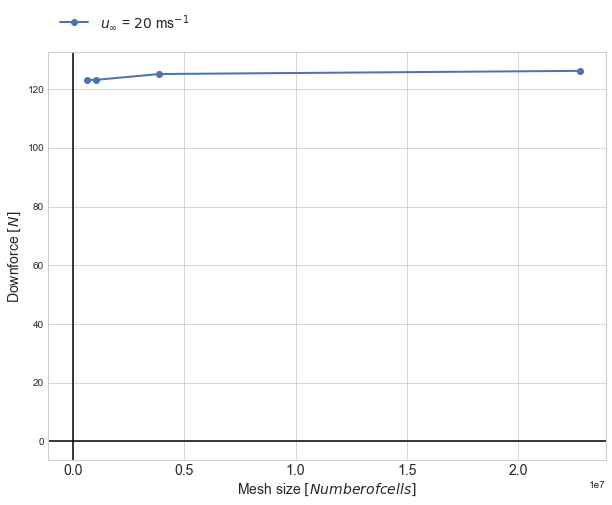
\includegraphics[width=\textwidth]{DFprmeshsize}
    \caption{Normalized downforce as a function of mesh size. Plotted to see the convergence towards the same force.}
    \label{fig:DFprmeshsize}
  \end{figure}

  Generating a mesh of correct size is done by sampling downforce over a range of mesh sizes. In figure \ref{fig:DFprmeshsize}, the normalized downforce is plotted as a function of the mesh size. The mesh independence study shows that the function converges to acceptable levels near the mesh size $\SI{.4E7}{}$, and serves to be a good compromise between results and computing time.

\section{Optimizing the Rear Wing}

  As mentioned in chapter \ref{chap:conceptdesign}, there's a large variation in parameters to optimize for. Numerical optimization has been done on end plates size and relative position of the two wing elements.


  \subsection{Verification of Simulation Results}
  \label{sec:simulationcomparison}

  Comparison with wind tunnel test.

  \subsubsection{Evaluation of Verification Simulation}

  \begin{figure}
    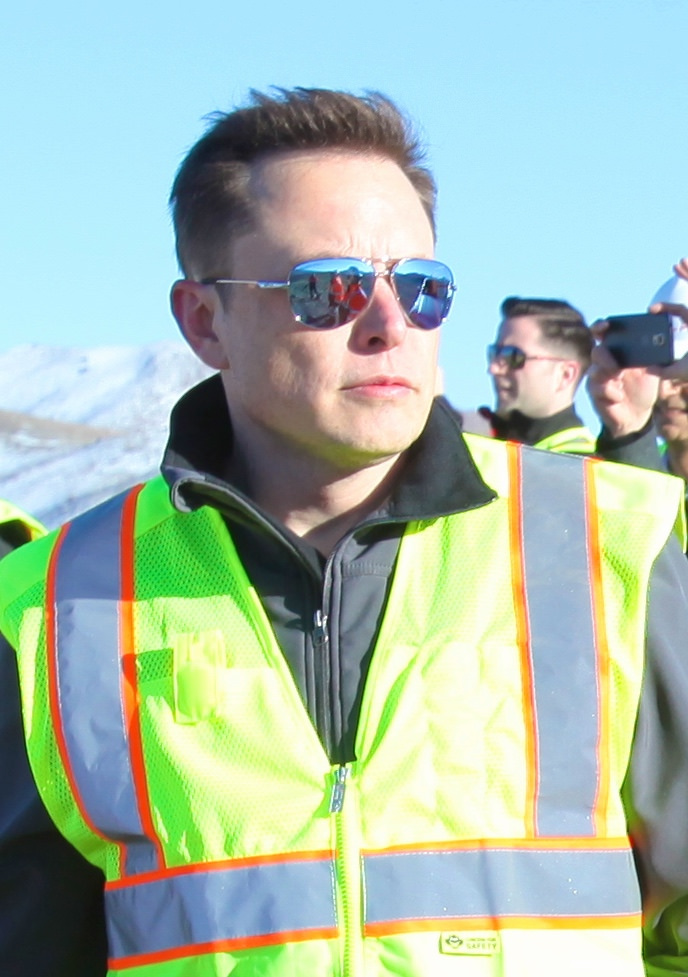
\includegraphics[width=\textwidth]{elon6}
    \caption{The simulation of the down scaled wing in the wind tunnel.}
    \label{fig:scalewingwindtunnelsim}
  \end{figure}

  \subsection{Multi-Element Wing Optimization}
  The influence of the two wing elements relative position on lift was examined to optimize the downforce the rear wing provides to the car at a given velocity. This relative position optimization was performed in the software package \emph{MultiElements Airfoils} provided from \emph{Hanley Innovations}. A scatterplot of the relative position is seen in figure \ref{fig:multieleoptimization}. The trailing edge of the first element is seem as the dark lines, and the position of the second elements leading edge is plotted, where the resulting lift coefficient is embedded as color. The redder the better lift coefficient. After sweeping, a maximum lift of $C_L = 2.60$  at $u = \SI{15}{\metre\per\second}$. is found with the leading edge of the secondary element placed at $x=\SI{0.5}{\metre},y=\SI{-0.01}{\metre}$ relative to the leading edge of the main element.

  \begin{figure}
    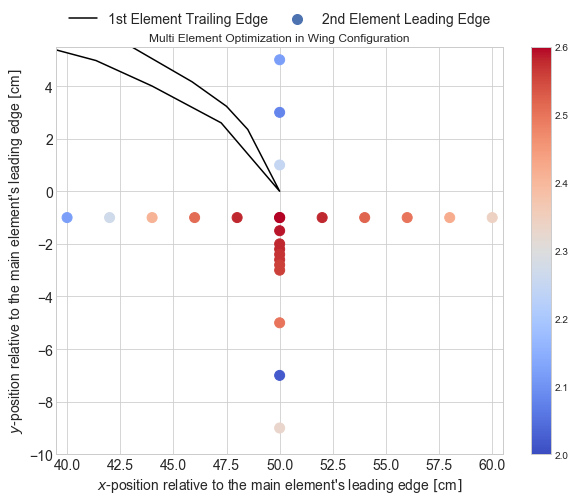
\includegraphics[width=\textwidth]{multieleoptimization2}
    \caption{Optimization of the two element wing. The redder the dots, the higher the lift coefficient.}
    \label{fig:multieleoptimization}
  \end{figure}

\section{Results}
